% M.ahmadi 1395.11.28   edit: 1400.07.25
% @Tex_Ahmadi 
% دو بار پردازش با زی‌لاتک
\PassOptionsToPackage{pdfpagemode=FullScreen,hyperfootnotes=false}{hyperref}
\documentclass[10pt,xcolor=dvipsnames]{beamer}

%\usepackage{amsmath,amssymb,amsfonts} 
\usepackage{etoolbox} 
\usepackage{tikz} 
\usepackage{graphicx}
\usepackage{listings}
\usepackage{ptext}

\usetheme{Warsaw}
\usefonttheme{serif,professionalfonts}
\usecolortheme[named=blue]{structure}
\setbeamercovered{transparent}

%%%%%%%%%%%%
\newlength\SubHt
\settoheight\SubHt{\usebeamerfont{subsection in head/foot}S}
\newlength\SubDh
\settodepth\SubDh{\usebeamerfont{subsection in head/foot}g}

\makeatletter
\setbeamertemplate{headline}
{%
  \leavevmode%
  \begin{beamercolorbox}[wd=.5\paperwidth,ht=1.5\SubHt,dp=1.5\SubDh]{section in head/foot}%
    \insertsectionnavigationhorizontal{.5\paperwidth}{\hskip0pt plus1filll}{}%
  \end{beamercolorbox}%
  \begin{beamercolorbox}[wd=.5\paperwidth,ht=1.5\SubHt,dp=1.5\SubDh]{subsection in head/foot}%
    \insertsubsectionnavigationhorizontal{.5\paperwidth}{}{\hskip0pt plus1filll}%
  \end{beamercolorbox}%
}
\makeatother

%%%%%%%%%%%%
% برای قرار گرفتن شماره اسلاید
\expandafter\def\expandafter\insertshorttitle\expandafter{%
  \insertshorttitle\hfill%
 \inserttotalframenumber\,/\,\insertframenumber}
 %%%%%%%%%%%%%%
 %توجه: بسته هایی که نیاز هست قبل از بسته زی‌پرشین نوشته شود.
\usepackage{xepersian}
\settextfont{XB Zar}
\setlatintextfont{Times New Roman}
\setdigitfont{Yas}

\defpersianfont\nas[Scale=1.5]{IranNastaliq}
\defpersianfont\xb[Scale=1.3]{XB Zar}
\deflatinfont\tnr[Scale=1.2]{Times New Roman}
%\linespread{1.2} 
% دستورات مورد نیاز برای استفاده از کلاس بیمر در command نوشته شده
%
% M.ahmadi 1395.11.08, copy of:
% http://qa.parsilatex.com/14100
% http://qa.parsilatex.com/14148
%%%%%%%%%%%%%%%%%
\makeatletter
\define@key{beamercolbox}{left}[0pt]{\def\beamer@colbox@rs{0pt}\def\beamer@colbox@ls{#1 plus1fill}}
\makeatother
%%%%%%%%%%%%%%%%%
\makeatletter
\expandafter\let\csname beamer@@tmpop@itemize item@default\endcsname\relax
\expandafter\let\csname beamer@@tmpop@itemize subitem@default\endcsname\relax
\expandafter\let\csname beamer@@tmpop@itemize subsubitem@default\endcsname\relax

\defbeamertemplate*{itemize item}{default}{\scriptsize\raise1.25pt\hbox{\donotcoloroutermaths$\blacktriangleleft$}}
\defbeamertemplate*{itemize subitem}{default}{\tiny\raise1.5pt\hbox{\donotcoloroutermaths$\blacktriangleleft$}}
\defbeamertemplate*{itemize subsubitem}{default}{\tiny\raise1.5pt\hbox{\donotcoloroutermaths$\blacktriangleleft$}}

\bidi@patchcmd{\@listi}{\leftmargin}{\rightmargin}{}{}
\let\@listI\@listi
\bidi@patchcmd{\@listii}{\leftmargin}{\rightmargin}{}{}
\bidi@patchcmd{\@listiii}{\leftmargin}{\rightmargin}{}{}
\bidi@patchcmd{\beamer@enum@}{\raggedright}{\raggedleft}{}{}
\bidi@patchcmd{\@@description}{\raggedright}{\raggedleft}{}{}
\bidi@patchcmd{\@@description}{\leftmargin}{\rightmargin}{}{}

\renewcommand{\itemize}[1][]{%
  \beamer@ifempty{#1}{}{\def\beamer@defaultospec{#1}}%
  \ifnum \@itemdepth >2\relax\@toodeep\else
    \advance\@itemdepth\@ne
    \beamer@computepref\@itemdepth% sets \beameritemnestingprefix
    \usebeamerfont{itemize/enumerate \beameritemnestingprefix body}%
    \usebeamercolor[fg]{itemize/enumerate \beameritemnestingprefix body}%
    \usebeamertemplate{itemize/enumerate \beameritemnestingprefix body begin}%
    \list
      {\usebeamertemplate{itemize \beameritemnestingprefix item}}
      {\def\makelabel##1{%
          {%
            \hss\llap{{%
                \usebeamerfont*{itemize \beameritemnestingprefix item}%
                \usebeamercolor[fg]{itemize \beameritemnestingprefix item}##1}}%
          }%
        }%
      }
  \fi%
  \beamer@cramped%
  \raggedleft%
  \beamer@firstlineitemizeunskip%
}
\makeatother
\hypersetup{pdfinfo={Author:={M.Ahmadi 1400-07-25}}}
%%%%%%%%%%%%%%%%%
\makeatletter
\bidi@undef\beamer@@tmpop@footnote@default
\defbeamertemplate*{footnote}{default}
{
  \parindent 1em\noindent%
  \raggedleft
  \hbox to 1.8em{\hfil\insertfootnotemark}\insertfootnotetext\par%
}
\defbeamertemplate*{LTRfootnote}{default}
{
  \parindent 1em\noindent%
  \raggedright
  \hbox to 1.8em{\hfil\insertfootnotemark}\latinfont\insertfootnotetext\par%
}
\footdir@temp\footdir@ORG@bidi@beamer@framefootnotetext\beamer@framefootnotetext{R}
\let\@footnotetext=\beamer@framefootnotetext
\let\@RTLfootnotetext\@footnotetext
\def\@makeLTRfntext#1{%
  \def\insertfootnotetext{#1}%
  \def\insertfootnotemark{\@makefnmark}%
  \usebeamertemplate***{LTRfootnote}}
\newcommand<>\beamer@frameLTRfootnotetext[1]{%
  \global\setbox\beamer@footins\vbox{\@RTLfalse%
    \hsize\framewidth
    \textwidth\hsize
    \columnwidth\hsize
    \unvbox\beamer@footins
    \reset@font\footnotesize
    \@parboxrestore
    \protected@edef\@currentlabel
         {\csname p@footnote\endcsname\@thefnmark}%
    \color@begingroup
      \uncover#2{\@makeLTRfntext{%
        \rule\z@\footnotesep\ignorespaces#1\@finalstrut\strutbox}}%
    \color@endgroup}}
\footdir@temp\footdir@ORG@bidi@beamer@frameLTRfootnotetext\beamer@frameLTRfootnotetext{L}
\let\@LTRfootnotetext=\beamer@frameLTRfootnotetext
\makeatother
%%%%%%%%%%%%%%
\makeatletter
\renewenvironment{beamercolorbox}[2][]{%
  \begingroup%
    \def\beamer@colbox@coladd{0pt}%
    \def\beamer@vmode{\leavevmode}%
    \setkeys{beamercolbox}{%
      wd=\textwidth,ht={},dp={},%
      rightskip=0pt,leftskip=0pt plus1fil,%
      sep=0pt,colsep=0pt,colsep*=0pt,%
      shadow=false,rounded=false,ignorebg=false}%
    \setkeys{beamercolbox}{#1}%
    \ifbeamercolorempty[bg]{#2}{\@tempswafalse}{\@tempswatrue}%
    \ifbeamer@colbox@ignorebg\@tempswafalse\fi%
    \def\beamer@colbox@color{#2}%
    \hsize=\beamer@colbox@wd%
    \setbox\beamer@tempbox=\hbox\bgroup\vbox\bgroup%
      \leftskip=\beamer@colbox@ls%
      \advance\leftskip by\beamer@colbox@sep%
      \rightskip=\beamer@colbox@rs%
      \advance\rightskip by\beamer@colbox@sep%
      \ifbeamer@colbox@ignorebg%
        \colorlet{beamer@temp@color}{bg}%
        \usebeamercolor[fg]{#2}%
        \colorlet{bg}{beamer@temp@color}%
      \else%
        \usebeamercolor[fg]{#2}%
      \fi%
      \if@tempswa%
        \advance\leftskip by\beamer@colbox@colsep%
        \advance\rightskip by\beamer@colbox@colsep%
        \ifdim\beamer@colbox@colsep=0pt\else\vskip\beamer@colbox@colsep\fi%
        \ifdim\beamer@colbox@colseps=0pt\else\vskip\beamer@colbox@colseps\fi%
      \fi%
      \ifdim\beamer@colbox@sep=0pt\else\vskip\beamer@colbox@sep\fi%
      \beamer@vmode\ignorespaces}{%
      \ifdim\beamer@colbox@sep=0pt\else\vskip\beamer@colbox@sep\fi%
      \if@tempswa\ifdim\beamer@colbox@colsep=0pt\else\vskip\beamer@colbox@colsep\fi\fi%
      \if@tempswa\ifdim\beamer@colbox@colseps=0pt\else\vskip\beamer@colbox@colseps\fi\fi%
    \egroup\egroup%
    \wd\beamer@tempbox=\hsize%
    \@tempdima=\wd\beamer@tempbox%
    \ifx\beamer@colbox@ht\@empty%
    \else%
      \ht\beamer@tempbox=\beamer@colbox@ht%
    \fi%
    \ifx\beamer@colbox@dp\@empty%
    \else%
      \dp\beamer@tempbox=\beamer@colbox@dp%
    \fi%
    \ifbeamer@colbox@rounded%
      \if@tempswa%
        \begin{beamerboxesrounded}[%
          shadow=\beamer@colbox@shadow,%
          lower=\beamer@colbox@color,%
          upper=normal text,%
          width=\beamer@colbox@wd]{}%
          \box\beamer@tempbox%
        \end{beamerboxesrounded}%
      \else%
        \ifdim\@tempdima>\textwidth%
          \setbox\beamer@tempbox=\hbox to\textwidth{\hss\box\beamer@tempbox\hss}%
        \fi%
        \box\beamer@tempbox%
      \fi%
    \else%
      \if@tempswa\setbox\beamer@tempbox=\hbox{\vbox{%
        \usebeamercolor{\beamer@colbox@color}%
        \advance\hsize by \beamer@colbox@colseps\relax%
        \advance\hsize by \beamer@colbox@colseps\relax%
        \hskip-\beamer@colbox@colseps%
        \fboxsep=0pt\colorbox{bg}{%
          \hskip\beamer@colbox@colseps%
          \hbox{\box\beamer@tempbox}%
          \hskip\beamer@colbox@colseps%
        }%
        \hskip-\beamer@colbox@colseps%
      }}\fi%
      \ifdim\@tempdima>\textwidth%
        \setbox\beamer@tempbox=\hbox to\textwidth{\hskip0pt minus\beamer@leftmargin\relax\box\beamer@tempbox\hskip0pt minus\beamer@rightmargin\relax}%
      \fi%
      \box\beamer@tempbox%
    \fi%
  \endgroup%
}
\makeatother
%%%%%%%%%%%%%%%%%%%%%%%
\makeatletter
\long\def\beamer@newenvnoopt#1#2#3#4{%
  \expandafter\renewcommand\expandafter<\expandafter>\csname#1\endcsname[#2]{#3}%<- here
  \expandafter\long\expandafter\def\csname end#1\endcsname{#4}%
}
\long\def\beamer@newenvopt#1#2[#3]#4#5{%
  \expandafter\renewcommand\expandafter<\expandafter>\csname#1\endcsname[#2][#3]{#4}%<- here
  \expandafter\long\expandafter\def\csname end#1\endcsname{#5}%
}
\renewcommand<>\beamer@columncom[2][\beamer@colmode]{%
  \beamer@colclose%
  \def\beamer@colclose{\end{minipage}\hfill\end{actionenv}\ignorespaces}%
\begin{actionenv}#3%
  \setkeys{beamer@col}{#1}%
  \begin{minipage}[\beamer@colalign]{#2}%
    \leavevmode\raggedleft\beamer@colheadskip\ignorespaces}
\renewenvironment<>{columns}[1][]{%
  \begin{actionenv}#2%
  \def\beamer@colentrycode{%
    \hbox to\textwidth\bgroup%
    \leavevmode%
    \hskip-\beamer@leftmargin%
    \nobreak%
    \beamer@tempdim=\textwidth%
    \advance\beamer@tempdim by\beamer@leftmargin%
    \advance\beamer@tempdim by\beamer@rightmargin%
    \hbox to\beamer@tempdim\bgroup%
    \hbox{}\hfill\ignorespaces}%
  \def\beamer@colexitcode{\egroup%
    \nobreak%
    \hskip-\beamer@rightmargin\egroup}%
  \ifbeamer@centered\setkeys{beamer@col}{c}\else\setkeys{beamer@col}{t}\fi%
  \setkeys{beamer@col}{#1}%
  \par%
  \leavevmode\beamer@colentrycode%
  \def\beamer@colclose{}\ignorespaces}%
  {\beamer@colclose\def\beamer@colclose{}\beamer@colexitcode\end{actionenv}}%
\makeatother
%%%%%%%%%%%%%%%%
\makeatletter
\expandafter\let\csname beamer@@tmpop@frametitle@shadow theme\endcsname\relax
\defbeamertemplate*{frametitle}{shadow theme}
{%
  \nointerlineskip%
  \vskip-2pt%
  \hbox{\leavevmode
    \advance\beamer@leftmargin by -12bp%
    \advance\beamer@rightmargin by -12bp%
    \beamer@tempdim=\textwidth%
    \advance\beamer@tempdim by \beamer@leftmargin%
    \advance\beamer@tempdim by \beamer@rightmargin%
    \hskip-\Gm@lmargin\hbox{%
      \setbox\beamer@tempbox=\hbox{\begin{minipage}[b]{\paperwidth}%
          \vbox{}\vskip-.75ex%
          \rightskip0.3cm
          \leftskip0.3cm plus1fil\leavevmode
          \insertframetitle%
          \ifx\insertframesubtitle\@empty%
            \strut\par%
          \else
            \par{\usebeamerfont*{framesubtitle}{\usebeamercolor[fg]{framesubtitle}\insertframesubtitle}\strut\par}%
          \fi%
          \nointerlineskip
          \vbox{}%
          \end{minipage}}%
      \beamer@tempdim=\ht\beamer@tempbox%
      \advance\beamer@tempdim by 2pt%
      \begin{pgfpicture}{0pt}{0pt}{\paperwidth}{\beamer@tempdim}
        \usebeamercolor{frametitle right}
        \pgfpathrectangle{\pgfpointorigin}{\pgfpoint{\paperwidth}{\beamer@tempdim}}
        \pgfusepath{clip}
        \pgftext[left,base]{\pgfuseshading{beamer@frametitleshade}}
      \end{pgfpicture}
      \hskip-\paperwidth%
      \box\beamer@tempbox%
    }%
    \hskip-\Gm@rmargin%
  }%
  \nointerlineskip
    \vskip-0.2pt
    \hbox to\textwidth{\hskip-\Gm@lmargin\pgfuseshading{beamer@topshade}\hskip-\Gm@rmargin}
    \vskip-2pt
}
\makeatother
%%%%%%%%%%%%%%%%%%
\makeatletter
\expandafter\let\csname beamer@@tmpop@section in toc@ball\endcsname\relax
\defbeamertemplate{section in toc}{ball}
{\leavevmode\rightskip=2.75ex%
  \llap{%
    \normalsize%
    \begin{pgfpicture}{-1ex}{-0.7ex}{1ex}{1ex}
      \pgftext{\beamer@usesphere{section number projected}{tocsphere}}
      \pgftext{%
        \usebeamerfont*{section number projected}%
        \usebeamercolor{section number projected}%
        \color{fg!90!bg}%
        \inserttocsectionnumber}
    \end{pgfpicture}%
    \kern1.25ex}%
  \inserttocsection\par
}
[action]
{\setbeamerfont{section number projected}{size=\scriptsize}}
\expandafter\let\csname beamer@@tmpop@subsection in toc@ball\endcsname\relax
\defbeamertemplate{subsection in toc}{ball}
{\leavevmode\rightskip=5ex%
  \llap{\raise0.1ex\beamer@usesphere{subsection number projected}{bigsphere}\kern1ex}%
  \inserttocsubsection\par%
}
\expandafter\let\csname beamer@@tmpop@subsubsection in toc@ball\endcsname\relax
\defbeamertemplate{subsubsection in toc}{ball}
{\leavevmode\normalsize\usebeamerfont{subsection in
    toc}\rightskip=7ex\usebeamerfont{subsubsection in toc}%
  \llap{\beamer@usesphere{subsubsection number projected}{bigsphere}\kern0.75ex}%
  \inserttocsubsubsection\par%
}
\setbeamertemplate{sections/subsections in toc}[ball]
\makeatother
\defpersianfont\nast[Scale=1.5,ExternalLocation]{IranNastaliq} 
%+++++++++++++++++++++++++++
% متلب
\definecolor{mygreen}{RGB}{28,172,0} 
\definecolor{mylilas}{RGB}{170,55,241}
\lstset{language=Matlab,
    breaklines=true,basicstyle=\ttfamily\scriptsize,
    morekeywords={matlab2tikz},
    keywordstyle=\color{blue},
    morekeywords=[2]{1}, keywordstyle=[2]{\color{black}},
    identifierstyle=\color{black},
    stringstyle=\color{mylilas},
    commentstyle=\color{mygreen},
    showstringspaces=false
}
%++++++++++++
%برای شماره خوردن قضیه،...
\setbeamertemplate{theorems}[numbered]
%برای شماره خوردن عنوان جدول و شکل
\setbeamertemplate{caption}[numbered]
%محیط های قضیه، تعریف، مثال، لم، نتیجه و.... را با حرف اول کوچک  در فریم ها بنویسید. مثال
\providetranslation{Theorem}{قضیه}%{\large \bf قضیه}
\providetranslation{Definition}{تعریف}
\providetranslation{Example}{مثال}
\providetranslation{Lemma}{لم}
\providetranslation{Corollary}{نتیجه}
\providetranslation{Solution}{پاسخ}
\providetranslation{Problem}{مسئله}
\providetranslation{Fact}{حقیقت}
%
\newtheorem{proposition}[theorem]{گزاره}
\AtBeginEnvironment{proposition}{\setbeamercolor{block title}{fg=white,bg=structure.fg!75!black}}

%++++++++++++++++++++++++++++++ @Tex_Ahmadi
\raggedleft
%%%%%%%
\newcommand*{\co}[1]{\nast\textcolor{blue}{#1}}
%%%%
\title{یک اسلاید نمونه}
\subtitle{زیرعنوان اسلاید}
\author[مجتبیٰ احمدی]{\co{مجتبیٰ احمدی}
\\[.2cm]
\textcolor{red}{{\xb استاد راهنما}}:
\\[.2cm]
\co{جناب آقای}
}
\institute{دانشگاه: پیام‌نو‌ر مشگین شهر}
\date{\today}
%\date{28 بهمن 1395}
%%%%%%%%%%
\logo{
\includegraphics[scale=.02]{logo1.png} }
\newcommand{\nologo}{\setbeamertemplate{logo}{}}

\begin{document}

{\nologo
\begin{frame}[plain,noframenumbering]
%برای عدم نمایش نوار بالایی و پایین در فرم آپشن plain و برای اینکه جزء شماره اسلاید محسوب نشود آپشن فرم noframenumbering قرار داده شده است.
\centerline{
\includegraphics[width=\paperwidth,height=\paperheight]{besm.jpg}}
\end{frame}}
%%%%%%%%%%%%%%
\begin{frame}
\begin{picture}(0,0)
\put (0,-20){\centerline{
\includegraphics[width=1.3cm]{logo.jpg}}}
\end{picture}
\vskip 0.1 in
\maketitle
\end{frame}
%%%%%%%%%%%%%%
\begin{frame}{فهرست مطالب}
\tableofcontents
\end{frame}
%%%%%%%%%%%%%%%%%%
\section{قسمتی که در اینجاست}
\subsection{زیرقسمتی که در اینجاست}
\subsubsection{زیرزیرقسمتی که در اینجاست}

\begin{frame}
\frametitle{عنوان}
\framesubtitle{زیرعنوان}
\begin{definition}
این یک تعریف است 
\begin{align}
2x - 5y &=  8 \\ 
3x + 9y &=  -12
\end{align}
\end{definition}

\end{frame}
%%%%%%%%%%%%%%%%%%%
\begin{frame}
\ptext[1]
\begin{enumerate}
\item 
این یک متن است که در اینجا قرار می‌دهیم این یک متن است که در اینجا قرار می‌دهیم. این یک متن است که در اینجا قرار می‌دهیم. این یک متن است که در اینجا قرار می‌دهیم.
\end{enumerate}
\pause

\begin{itemize}
\item 
این یک متن است که در اینجا قرار می‌دهیم این یک متن است که در اینجا قرار می‌دهیم. این یک متن است که در اینجا قرار می‌دهیم. این یک متن است که در اینجا قرار می‌دهیم.
\end{itemize}

\begin{description}
\item[آزمایش]
این یک متن است که در اینجا قرار می‌دهیم این یک متن است که در اینجا قرار می‌دهیم. این یک متن است که در اینجا قرار می‌دهیم. این یک متن است که در اینجا قرار می‌دهیم.
\end{description}

\end{frame}
%%%%%%%%%%%%%%%%%%%%%%%%
\begin{frame}

\footnote{این یک زیرنویس پارسی است.}%

\LTRfootnote{This is a latin footnote.}%

\RTLfootnote{این هم زیرنویس پارسی دیگری است.}%

\footnote{این یک زیرنویس پارسی است.}

\end{frame}
%%%%%%%%%%%%%%%%%
\begin{frame}
\ptext[1]
\begin{definition}
این یک تعریف است
\end{definition}
\pause

\begin{theorem}
این یک قضیه است
\end{theorem}
\pause

\begin{proof}
این یک اثبات است.
\end{proof}
\pause

\begin{example}
این یک مثال است
\end{example}
\end{frame}
%++++++++
\begin{frame}{شمارش محیط‌ها}
\begin{definition}
این یک تعریف است
\begin{figure}
\centering

\includegraphics[scale=.02]{logo1.png} 
\caption{لوگو}
\end{figure}
\end{definition}
\pause

\begin{theorem}
این یک قضیه است
\end{theorem}
\pause

\begin{proof}
این یک اثبات است.
\end{proof}

\end{frame}
% 7
\begin{frame}
\begin{example}
این یک مثال است
\end{example}
\begin{corollary}
متن
\end{corollary}

\begin{proposition}
تست
\end{proposition}
\begin{lemma}
متن
\end{lemma}
\end{frame}
%++++++++
%%%%%%%%%%%%%%%%%%%%%%%
\section{بخش بعدی}
\subsection{زیربخش بعدی}
\subsubsection{زیرزیربخش بعدی}
\begin{frame}
\begin{columns} 
 \column{.5\textwidth}
ستون شماره ۱
\begin{latin}
This is a test as you can see
\end{latin}
 \column{.2\textwidth}
ستون شماره ۲
\column{0.3\textwidth}
ستون شماره ۳
\end{columns}

\begin{block}{فرمول ریاضی}
\begin{equation}
\sum_{i=1}^{n} i = \frac{n(n+1)}{2}
\end{equation}
\end{block}

\end{frame}
%%%%%%%%%%%%%%%%%%%%%%%%%%%
\begin{frame}{عنوان اسلاید این صفحه  که در اینجا قرار می‌گیرد}
\begin{example}
این یک مثال است.
\end{example}


\begin{definition}
این یک تعریف است.
\begin{itemize}\raggedright
\item 1
\item 2
\end{itemize}
\end{definition}

\begin{proof}
این یک اثبات است که در اینجا نوشته می‌شود و فقط مقدار بیشتر متن و متن که نوشته می‌شود تا بتوانیم به سطر بعدی برویم.
\end{proof}

\end{frame}
%%%%%%%%%%%%%%%%%%%%%%%%%
\begin{frame}[fragile]{کد متلب}
\textcolor{red}{توجه}:
برای نوشتن کد برنامه‌ای نیاز هست که آپشن فرم رو 
\lr{fragile}
قرار دهیم.
\begin{latin}
\begin{lstlisting}[frame=single,rulecolor=\color{magenta},numbers=left,numberstyle=\tiny]
%==================================================
% Author:M.Ahmadi                   date:1394.10.20
%                 http://matlabp.ir
%==================================================
% The numbers 1 to 9, to form a rhombus.
clc
n=9;
for i=1:n
  for k=n-1:-1:i
    fprintf(' ');
  end;
  for j=1:i
    fprintf('%d',j);
  end;
  for j=i-1:-1:1
    fprintf('%d',j);
  end;
  fprintf('\n');
end;
\end{lstlisting}
\end{latin}
\end{frame}
%%%%%%%%%
\setbeamertemplate{frametitle continuation}{\insertcontinuationcount}
%آپشن allowframebreaks برای شکستن مراجع قرار داده شده
\begin{frame}[allowframebreaks]{منابع}
\setbeamertemplate{bibliography item}{\insertbiblabel}
\begin{latin}
\begin{thebibliography}{9}
\bibitem{1}
Mojtaba Ahmadi.
 \newblock {The Math books and Examples of \LaTeX in Weblog}.
 \newblock \texttt{http://ahmadi1386.persianblog.ir/}, 1993/04/15.
\bibitem{2}
 Vafa Khalighi.
 \newblock {The XePersian Package, Persian for \LaTeX2e over \XeTeX}.
 \newblock \texttt{http://ctan.org/pkg/xepersian}, 2008.
 \bibitem{3}
 This is a test for break.  This is a test for break. 1
\bibitem{4}
 This is a test for break.  This is a test for break. 2
 \bibitem{5}
 This is a test for break.  This is a test for break. 3
 \bibitem{6}
 This is a test for break.  This is a test for break. 4
 \bibitem{7}
 This is a test for break.  This is a test for break. 5
\bibitem{8}
 This is a test for break.  This is a test for break. 6
 \bibitem{9}
 This is a test for break.  This is a test for break. 7
 \bibitem{10}
 This is a test for break.  This is a test for break. 8
 \bibitem{11}
 This is a test for break.  This is a test for break. 9
 \bibitem{12}
 This is a test for break.  This is a test for break. 10
 \bibitem{13}
 This is a test for break.  This is a test for break. 11
\end{thebibliography}
\end{latin}

\end{frame}
%
\usebackgroundtemplate{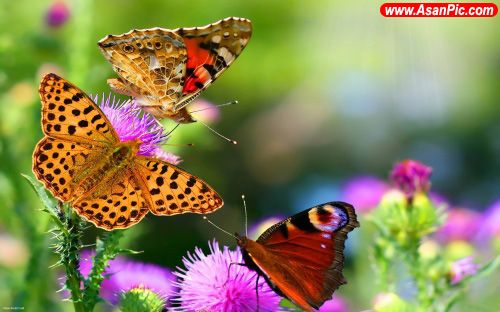
\includegraphics[width=\paperwidth,height=\paperheight]{20.jpg} }
\nologo
\begin{frame}
\begin{center}
\Huge {\nas
\textcolor{red}{با آرزوی موفقیت}}
\end{center}
\end{frame}

\end{document}
